% This example An LaTeX document showing how to use the l3proj class to
% write your report. Use pdflatex and bibtex to process the file, creating 
% a PDF file as output (there is no need to use dvips when using pdflatex).

% Modified 

\documentclass{l3proj}
\begin{document}
\title{Project Title}
\author{Michael Kilian \\
        Tony Lau \\
        Dan Tomosoiu \\
        Hector Grebbell \\
        Peeranat Fupongsiripan}
\date{13 March 2013}
\maketitle
\begin{abstract}

The abstract goes here

\end{abstract}
\educationalconsent
\tableofcontents
%==============================================================================
\chapter{Introduction}
\label{intro}

ALICE \cite{alice} was beginning to get very tired of sitting by her sister
on the bank and of having nothing to do: once or twice she had peeped into
the book her sister was reading, but it had no pictures or conversations in
it, ``and what is the use of a book,'' thought Alice, ``without pictures or
conversations?'

\begin{figure}
\begin{center}
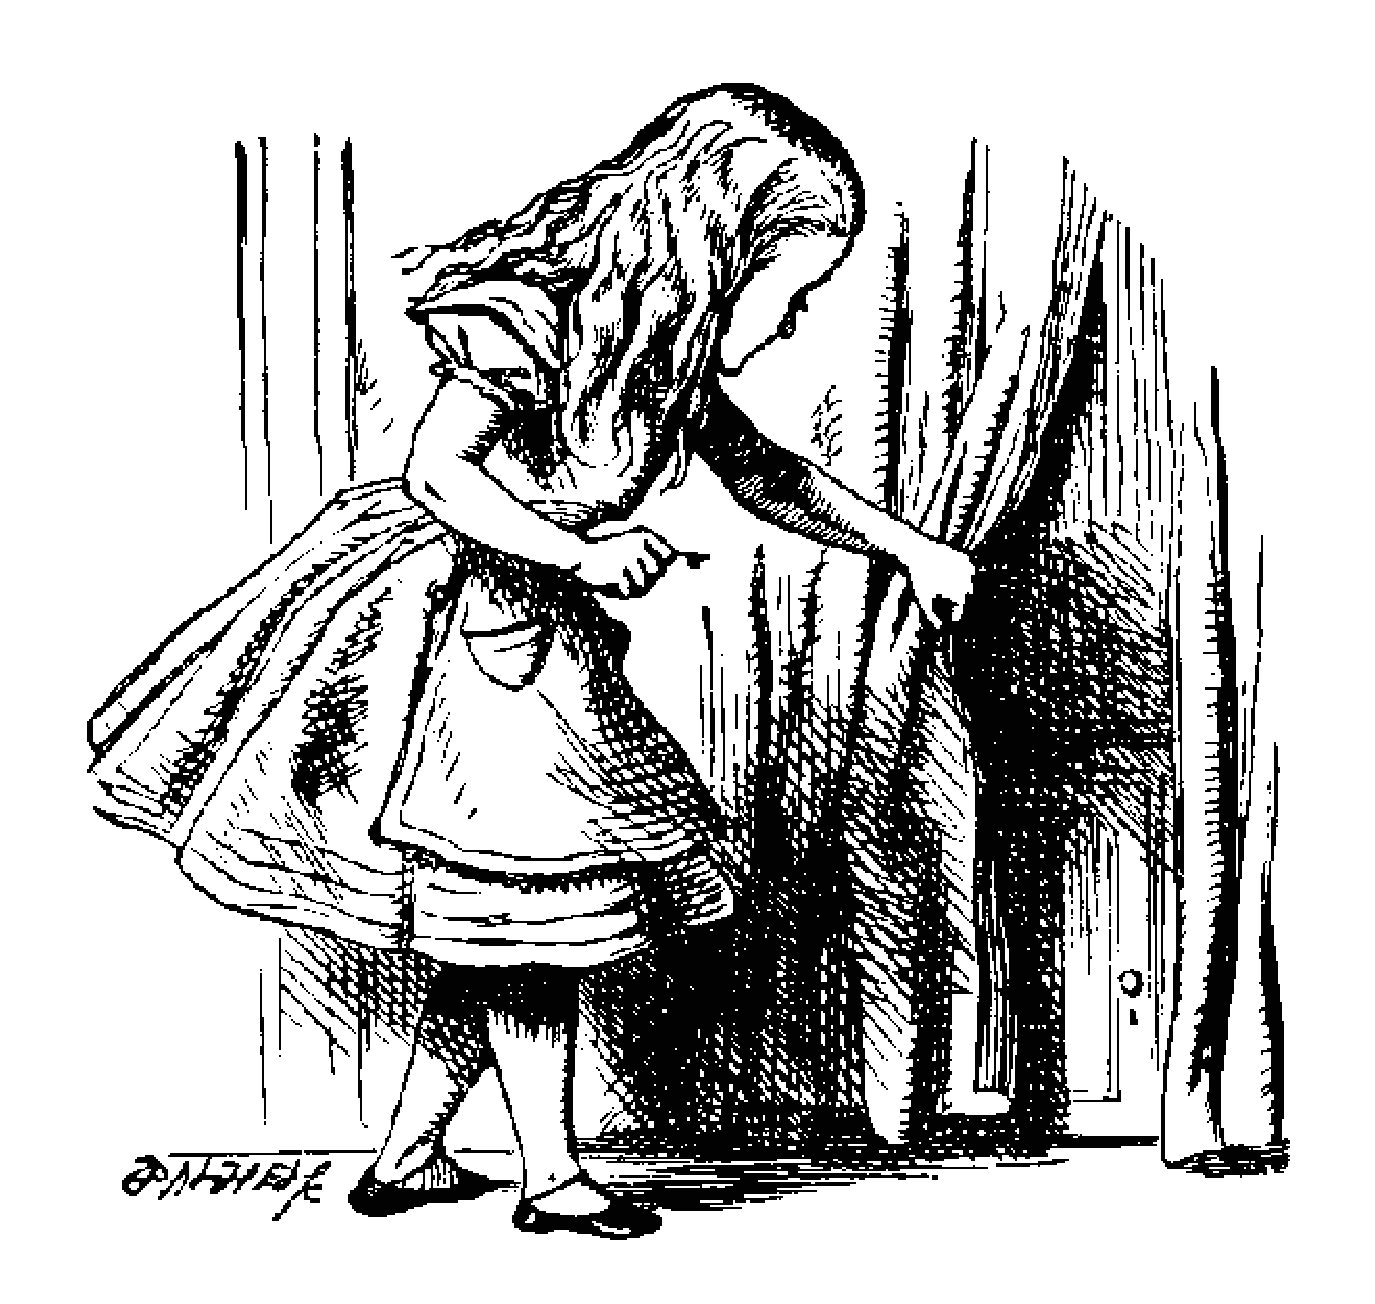
\includegraphics[width=7cm]{figures/alice}
\end{center}
\caption{Behind it was a little door}
\label{fig:alice}
\end{figure}

Alice opened the door and found that it led into a small passage.

%==============================================================================
\chapter{Research and Requirements}
\label{impl}

Requirements (chapter on its own?)

%------------------------------------------------------------------------------

%==============================================================================
\chapter{Design}
\label{design}

The following diagrams (especially figure \ref{fig:alice}) illustrate the
process...

%==============================================================================
\chapter{Implementation}
\label{impl}

In this chapter, we describe how the implemented the system.

%------------------------------------------------------------------------------
\section{User Interface}

Blah blah blah
Blah blah blah
Blah blah blah
Blah blah blah

% - - - - - - - - - - - - - - - - - - - - - - - - - - - - - - - - - - - - - - -
\subsection{Foo}

Blah blah blah
Blah blah blah
Blah blah blah
Blah blah blah

%------------------------------------------------------------------------------
\section{Database Model}

\begin{enumerate}
\item Blah blah blah
\item Blah blah blah
\item Blah blah blah
\item Blah blah blah
\end{enumerate}



%==============================================================================
\chapter{Evaluation}

We evaluated the project by...

%==============================================================================
\chapter{Conclusion}

A great project!

%==============================================================================
\section{Contributions}

Here we explain that Lewis Carroll wrote chapter \ref{intro}. John Wayne
was out riding his horse every day and didn't do anything. Marilyn Monroe
was great at getting the requirements specification and coordinating the
writing of the report. Betty Davis did the coding of the kernel of the
project, described in Chapter \ref{impl}.  James Dean handled the
multimedia content of the project.

%==============================================================================
\bibliographystyle{plain}
\bibliography{teamL_dissertation_2013}
\end{document}
